\documentclass{beamer}
\usetheme{metropolis}
\usepackage{graphicx}
\usepackage{amsmath}
\title{Digital Signal Processing: COSC390}
\author{Jordan Hanson}
\institute{Whittier College Department of Physics and Astronomy}

\begin{document}
\maketitle

\begin{frame}{Unit 1.2 Outline}
Previous lectures covered:
\begin{itemize}
\item Complex numbers 1: Arithmetic and some calculus (continuous and discete) ... see Chapter 30 of text
\end{itemize}
This lecture will cover:
\begin{itemize}
\item \alert{Complex numbers 2: The Fourier series and Fourier transform (continuous and discrete)}
\end{itemize}
Next lecture will cover:
\begin{itemize}
\item \textit{Time-permitting}: The Laplace transform (continuous and discrete)
\end{itemize}
\end{frame}

\section{Complex numbers 2: theory and examples}

\begin{frame}{Complex numbers 2: theory and examples}
Review: Let's work the following examples.
\begin{enumerate}
\item Let $z_1 = x_1 + j y_1$, and $z_2 = x_2 + j y_2$.  Simplify $z = \frac{z_1^* z_2}{|z_1|^2 + |z_2|^2}$ into real and imaginary parts.
\item Express $z$ in polar form and plot it for $x_1 = y_1 = 1.0$, and $x_2 = y_2 = -1.0$.
\item Express the function $v(t) = v_0 \cos(\omega t + \phi_0)$ as a phasor, and plot it.
\end{enumerate}
\end{frame}

\begin{frame}{Complex numbers 2: theory and examples}
The \alert{\textbf{Fourier series}} representation of a function $f(x)$ is written:
\begin{equation}
S(x) = \frac{A_0}{2}+\sum_{i=1}^{\infty} \left( A_n \cos(nx) + B_n \sin(nx) \right)
\end{equation}
with
\begin{align}
A_n &= \frac{1}{\pi} \int_0^{2\pi} f(x) \cos(nx) dx \\
B_n &= \frac{1}{\pi} \int_0^{2\pi} f(x) \sin(nx) dx
\end{align}
\end{frame}

\begin{frame}{Complex numbers 2: theory and examples}
Let's obtain the \alert{\textbf{Fourier series}} coefficients $A_n$ and $B_n$ for a square-wave signal:
\begin{equation}
f(x) = 1, ~~ 0 \leq x \leq \pi, ~~ 0,  \pi < x \leq 2\pi 
\end{equation}
(Observe on board).  The result: $A_0 = 1.0$, all other $A_n = 0$, odd $B_n$ values follow $2/(n\pi)$, even $B_n = 0$ as well. \\ \vspace{0.5cm}
Create octave code that plots this (see Moodle for example).  Initially, plot a solution that has the first 5 coefficients. \\ \vspace{0.5cm}
\alert{Plot a solution with the first 20 coefficients.}  \textit{Hint: can you find how to use the for-loop in octave?}
\end{frame}

\begin{frame}[fragile]{Complex numbers 2: theory and examples}
Let's obtain the \alert{\textbf{Fourier series}} coefficients $A_n$ and $B_n$ for a sawtooth-wave signal:
\begin{equation}
f(x) = x, ~~ -\pi < x < \pi
\end{equation}
Notice that (for technical reasons) we are always dealing with \textit{repeating signals}.
First obtain the coefficients $A_n$ and $B_n$ (we can use complex numbers to help with the integral). \\ \vspace{0.5cm}
\alert{Copy your previous octave code and modify it to plot this solution for the first 20 coefficients.}
\begin{verbatim}
for i=[1:n]
    ...
endfor
\end{verbatim}
\end{frame}

\begin{frame}[fragile]{Complex numbers 2: theory and examples}
\small
We now have a way to describe a \textit{continuous signal} \textbf{\alert{digitally.}} Ponder this for a moment.  How is this possible?  Aren't we representing an infinite quantity of information with a finite quantity? \\ \vspace{0.5cm}
\begin{figure}
\centering
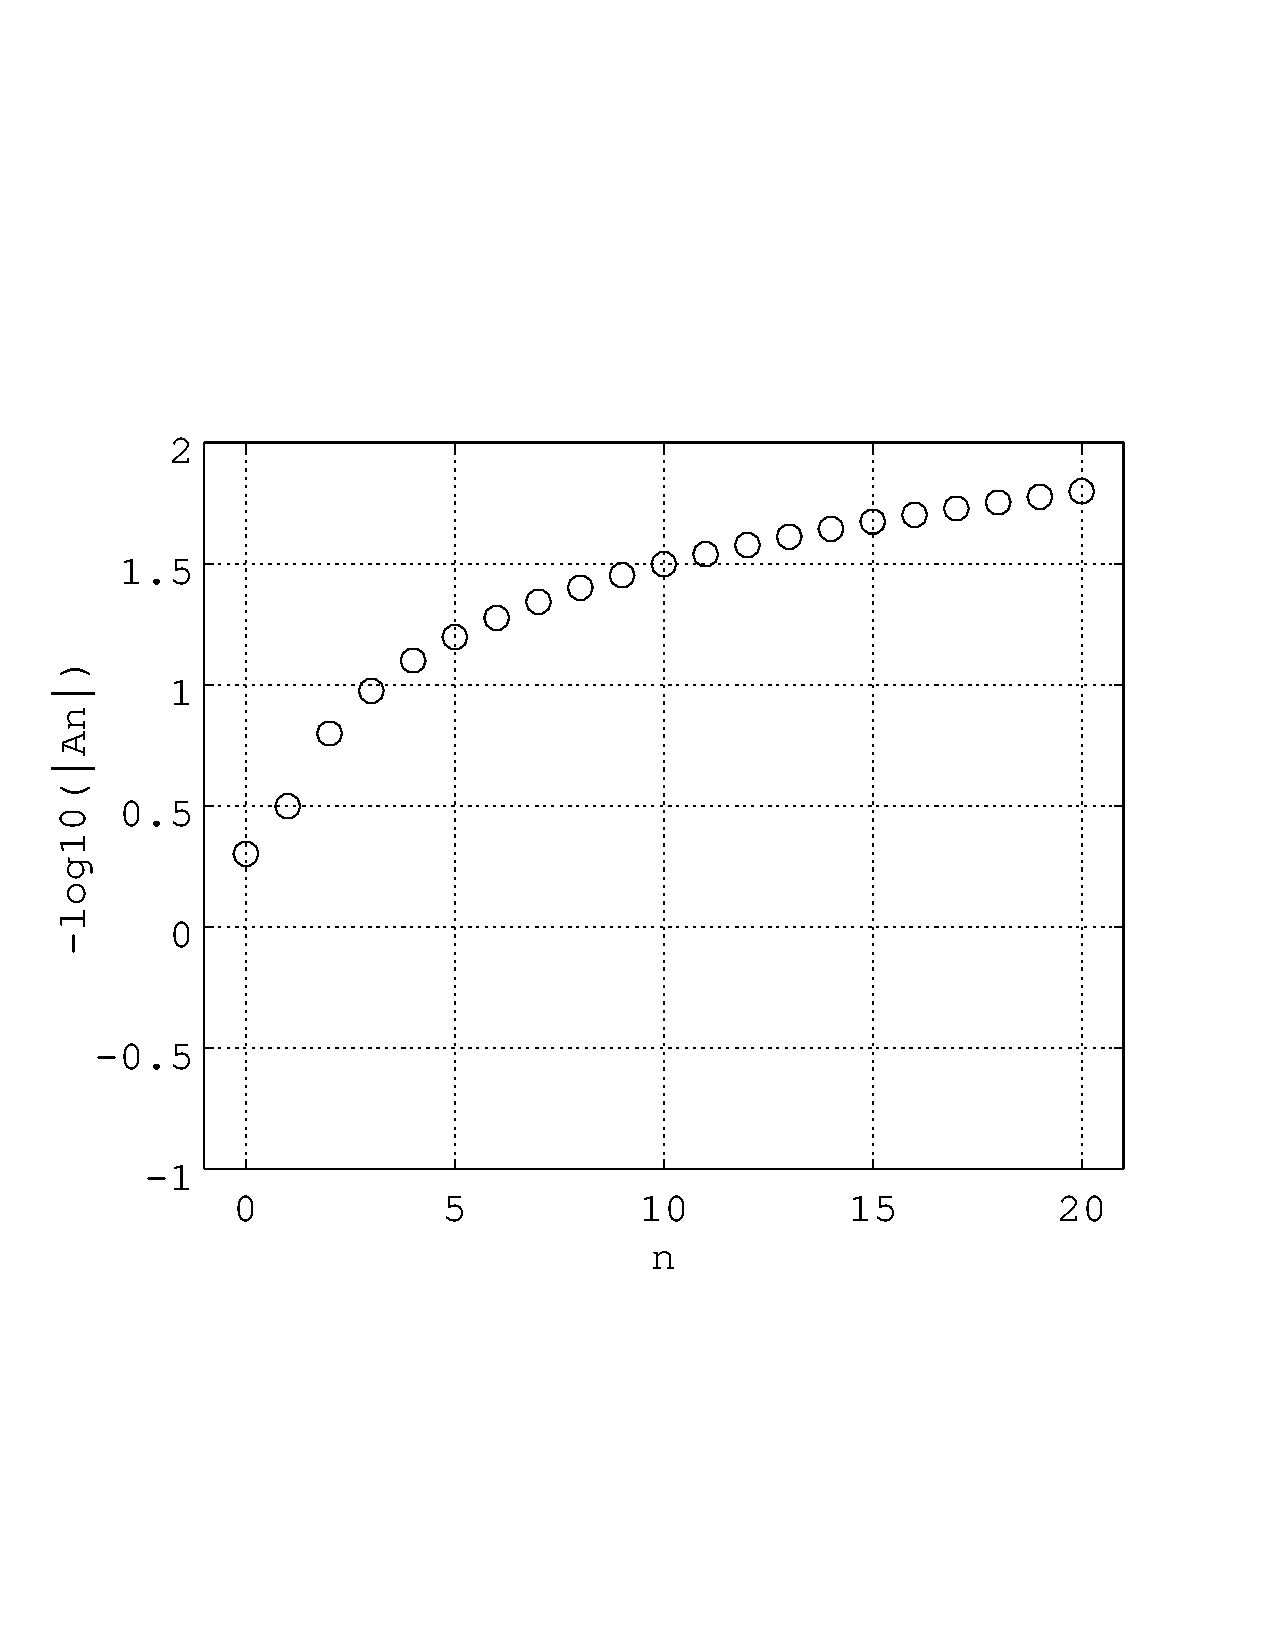
\includegraphics[width=0.5\textwidth,trim=1cm 6cm 1cm 7cm,clip=true]{figures/saw_coeff.pdf}
\caption{\label{fig:saw} The negative base-10 logarithm of the Fourier coefficients $A_n$ describing a saw-tooth wave.}
\end{figure}
\end{frame}

\begin{frame}[fragile]{Complex numbers 2: theory and examples}
\begin{figure}
\centering
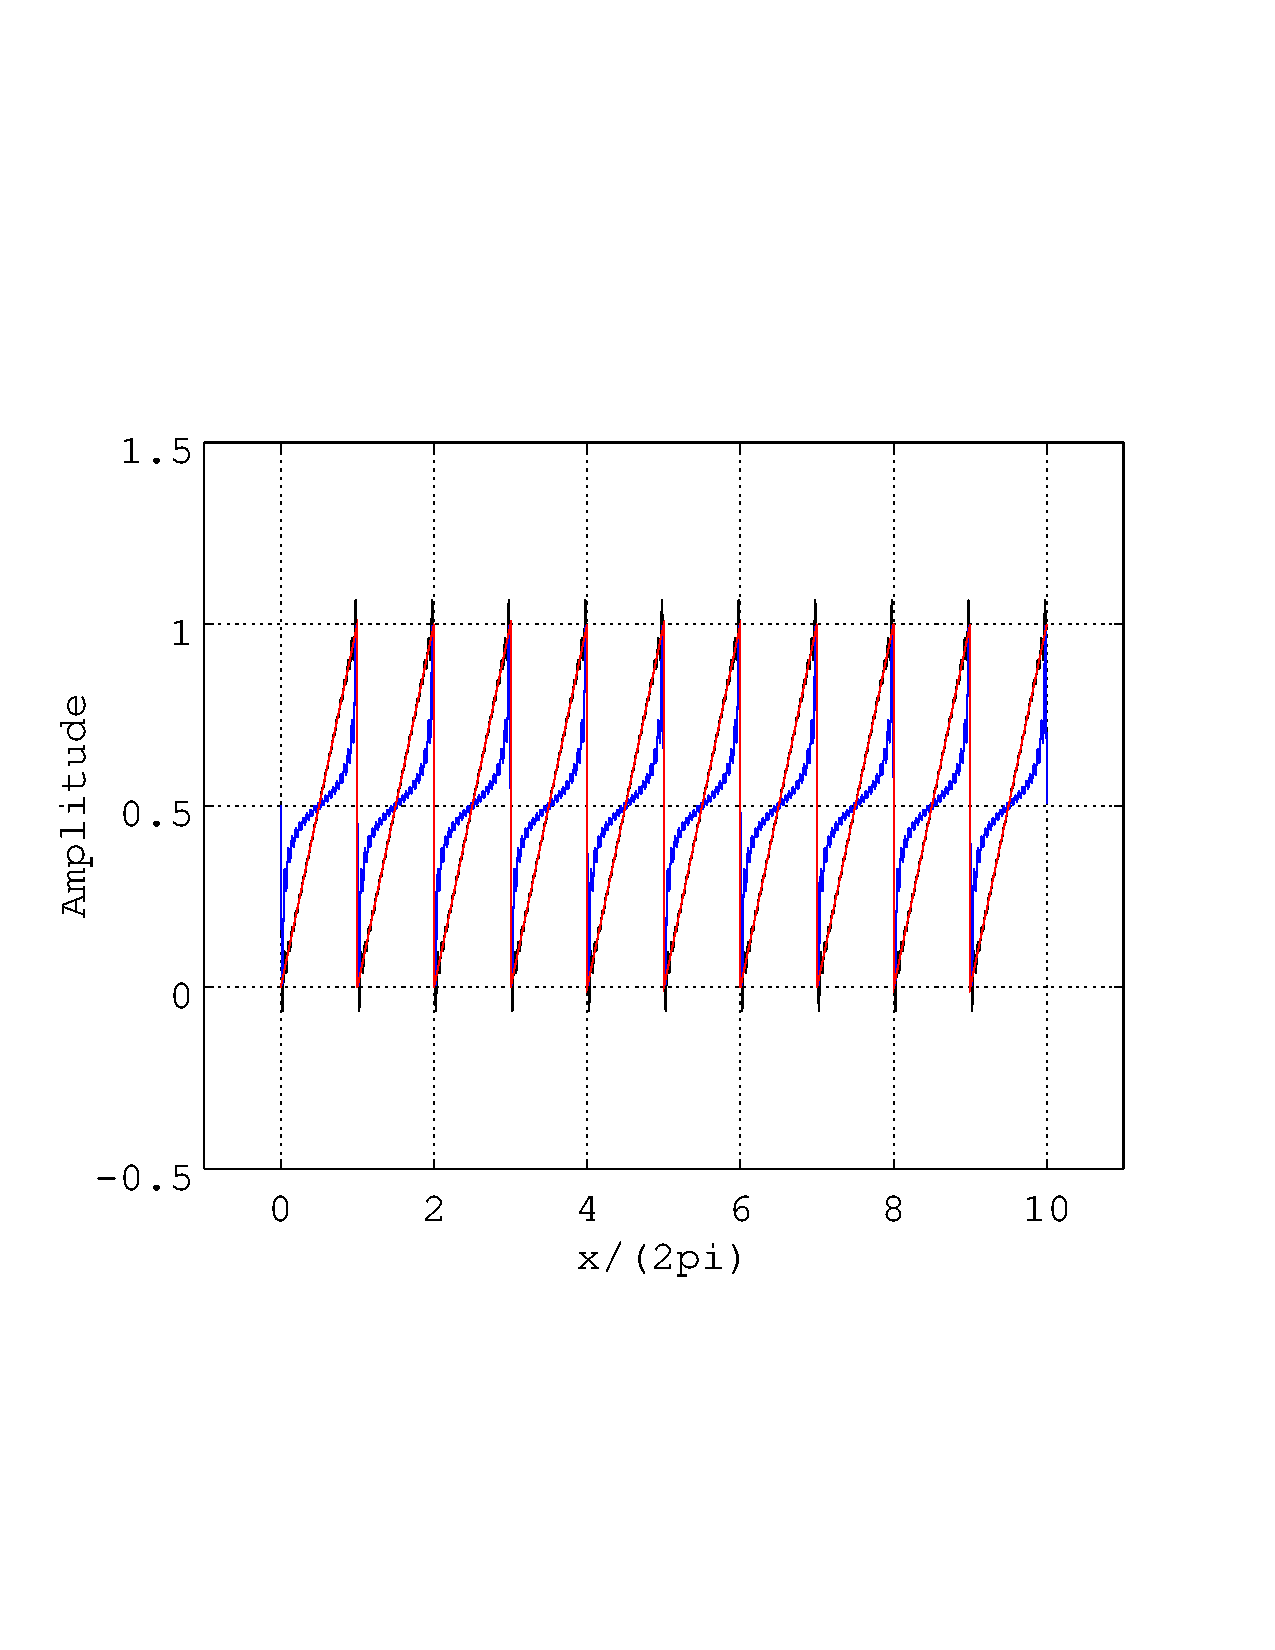
\includegraphics[width=0.5\textwidth,trim=1cm 6cm 1cm 7cm,clip=true]{figures/saw1.pdf}
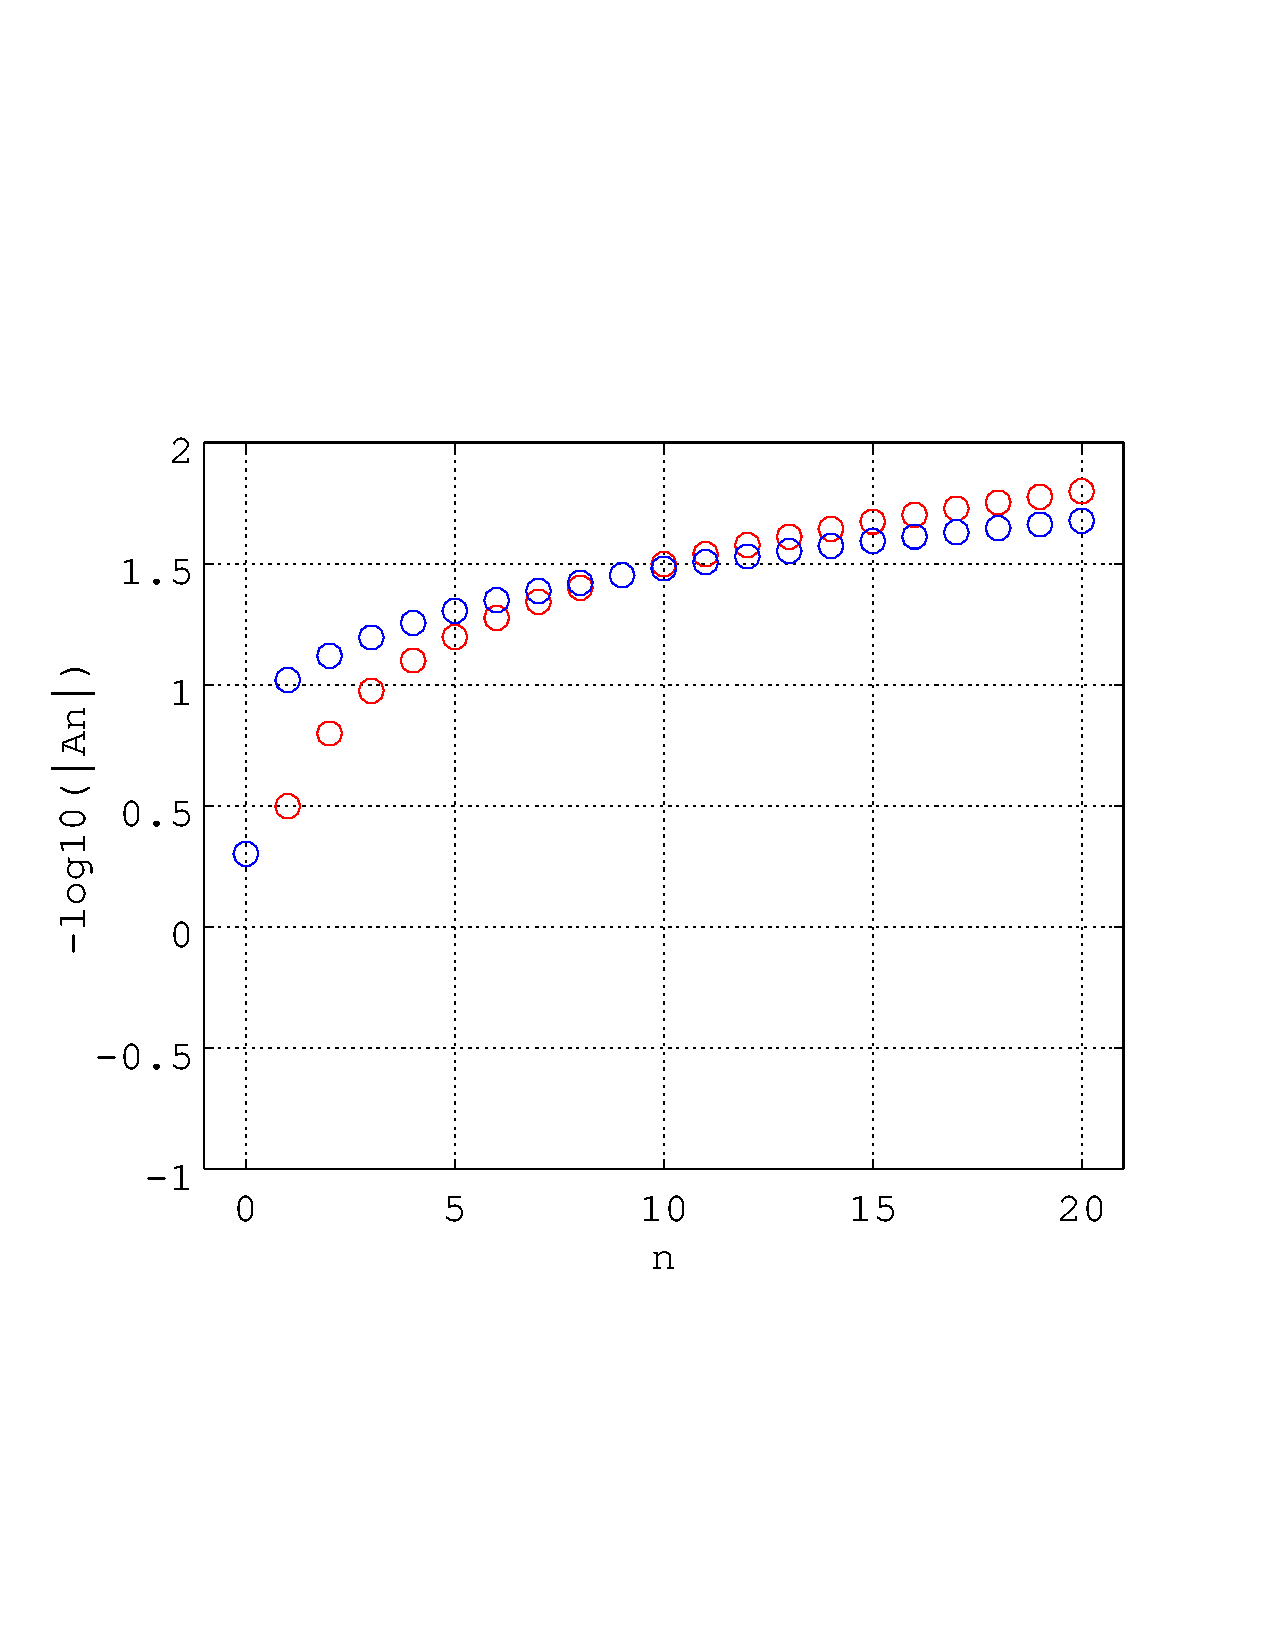
\includegraphics[width=0.5\textwidth,trim=1cm 6cm 1cm 7cm,clip=true]{figures/saw_coeff_mod.pdf}
\caption{\label{fig:saw2} A modification in the digital \textit{spectrum} (right) leads to a modification in the sampled signal (right).}
\end{figure}
\end{frame}

\begin{frame}[fragile]{Complex numbers 2: theory and examples}
The octave \textbf{play} and \textbf{audioplayer} command:
\begin{verbatim}
fs = 44000.0;
dt = 1/fs;
t = [0:dt:2.0];
v = 0.5*sin(2.0*pi*3000.0.*t);
player = audioplayer(v,fs,8);
play(player)
\end{verbatim}
These should define a digital waveform to play, and play it over the speakers.
\end{frame}

\begin{frame}[fragile]{Complex numbers 2: theory and examples}
Activity:
\begin{enumerate}
\item Create a sawtooth-wave and play it with octave.
\item Create a distorted sawtooth-wave and play it with octave.
\item Compare the sounds.  Why do they sound different?
\item Create a waveform that 
\item \alert{Bonus: write code that plays a short tune.}\footnote{This is more of a programming/engineering exercise than mathematics.}  How can you get multiple notes to play at once?  What is an \textbf{octave}, in the sense of musical notes and frequencies?
\end{enumerate}
\end{frame}

\begin{frame}[fragile]{Complex numbers 2: theory and examples}
\small
Notice that in order to \textit{plot} the sampled signal using a finite number of Fourier coefficients, we had to define $x$ as 
\begin{verbatim}
x = x_start:dx:x_end
\end{verbatim}
What happens in our code if we decrease the overall number of samples by increasing $dx$ while keeping the other two variables constant? \\ \vspace{0.5cm}
Try this with either your sound-playing code or code that plots sawtooth waves.  \textit{This is known as the sampling problem, and we will return to it in a moment.} \\ \vspace{0.5cm}
Finally, let's bring the concepts of \textit{sampling} and \textit{complex numbers} together, for the \textbf{\alert{Fourier transform}}.
\end{frame}

\begin{frame}[fragile]{Complex numbers 2: theory and examples}
First, let's split our representation of the function $f(t)$ with the Fourier series into two parts, absorb the constant into the first term, and re-scale by $1/\pi$:
\begin{equation}
f(t) = \frac{1}{\pi}\sum_{i=1}^N A_n \cos(nt) + \frac{1}{\pi}\sum_{i=1}^N B_n \sin(nt)
\end{equation}
The first term is the ``even'' term, and the second term is the ``odd'' term, because of the even-ness and odd-ness of the cosines and sines (hopefully this started to dawn on us in in the sawtooth and square-wave exercises).
\end{frame}

\begin{frame}[fragile]{Complex numbers 2: theory and examples}
\small
Now our coefficient equations read (because of the missing $\pi$):
\begin{align}
A_n &= \int f(t) \cos(nt) dt \\
B_n &= \int f(t) \sin(nt) dt
\end{align}
Consider the following function:
\begin{equation}
F(n) = A_n - j B_n = \int f(t) \cos(nt) dt - j \int f(t) \sin(nt) dt
\end{equation}
Integrals are \textit{linear}, in that they distribute over the same function:
\begin{equation}
F(n) = \int f(t) (\cos(nt) - j \sin(nt)) dt = \int f(t) \exp(-jnt) dt
\end{equation}
\end{frame}

\begin{frame}[fragile]{Complex numbers 2: theory and examples}
\small
Now we have:
\begin{equation}
F(n) = \int f(t) \exp(-jnt) dt
\end{equation}
\alert{Important question}: what are the units of $t$?  Don't they have to be unit-less?  Otherwise we cannot take the exponential of integers times seconds.  Let $t \rightarrow t/T$, where $T$ is the \textit{period}:
\begin{equation}
F(n) = \frac{1}{T}\int f(t) \exp(-jnt/T) dt
\end{equation}
Imagine a wave oscillating in the lowest \textit{harmonic}\footnote{Professor: draw a picture of this.}. The \textit{frequency} of the lowest harmonic is $f = 1/T$.  Suppose the integer $n$ \textit{selects} the harmonic (units: Hz):
\begin{equation}
f = \frac{n}{T}
\end{equation}
\end{frame}

\begin{frame}[fragile]{Complex numbers 2: theory and examples}
\small
Now let's have the integer select the harmonic, but in angular frequency:
\begin{equation}
\omega = 2\pi f = \frac{n}{T}
\end{equation}
This in turn causes the function $F(n)$ to be\footnote{Remember this integral is over a finite interval.  Let's call it $[-T,T]$.}
\begin{equation}
F(n) = \frac{1}{T}\int_{-T}^{T} f(t) \exp(-2j\pi f t) dt = \frac{1}{T}\int_{-T}^{T} f(t) \exp(-j\omega t) dt
\end{equation}
We can choose any high-frequency we wish by taking $n \rightarrow \infty$.  Currently, though, the lowest frequency we can get is for $n=1$, or $\omega = T^{-1}$.  If we let $T \rightarrow \infty$, then we can get any frequency, but that makes the limits of our integral infinite:
\begin{equation}
F(n) = \lim_{T\rightarrow \infty} \frac{1}{T}\int_{-T}^{T} f(t) \exp(-2j\pi f t) dt
\end{equation}
\end{frame}

\begin{frame}[fragile]{Complex numbers 2: theory and examples}
\small
For a special class of functions\footnote{Mumble mumble ... wait until you take quantum mechanics.} this integral is simply:
\begin{equation}
\boxed{
F(\omega) = \int_{-\infty}^{\infty} f(t) \exp(-j\omega t) dt}
\end{equation}
It turns out the inverse operation looks like:
\begin{equation}
\boxed{
F(t) = \frac{1}{2\pi} \int_{-\infty}^{\infty} F(\omega) \exp(j\omega t) d\omega)}
\end{equation}
Let's do some \textit{easy} examples together.  Let's obtain $F(\omega)$ for the following functions:
\begin{enumerate}
\item $f(t) = 1.0 ~~ |t| \leq T/2$
\item $f(t) = \exp(-t/\tau)$ for $t \geq 0$, zero everywhere else.
\end{enumerate}
\end{frame}

\begin{frame}[fragile]{Complex numbers 2: theory and examples}
\small
\begin{enumerate}
\item $T \left(\frac{\sin(x)}{x}\right)$, where $x = \frac{\omega T}{2}$
\item $\tau/(1+j\omega \tau)$
\end{enumerate}
\begin{enumerate}
\item Use octave to plot each result.
\item Modify the script so that the \textit{time-domain} signal and the \textit{frequency-domain} signal are plotted one above the other.
\end{enumerate}
To make multiple plots:
\begin{verbatim}
figure(1);
subplot(2,1,1)
plot(x,y);
subplot(2,1,2);
plot(x2,y2);
\end{verbatim}
\end{frame}

\begin{frame}[fragile]{Complex numbers 2: theory and examples}
\small
Now let's try a strange example.  Consider the \textit{delta-function}, or delta-distribution, defined by
\begin{equation}
f(t_0) = \int_{-\infty}^{\infty} \delta(t-t_0) f(t) dt
\end{equation}
In other words, the $\delta$-function is 1.0 at the point $t_0$, but zero everywhere else\footnote{...sort of, but don't ask questions.}.  What is the Fourier transform of the function $a\delta(t-t_0)$?
\begin{equation}
F(\omega) = \int_{-\infty}^{\infty} a\delta(t-t_0) \exp(-j\omega t) dt
\end{equation}
\end{frame}

\begin{frame}[fragile]{Complex numbers 2: theory and examples}
\small
Sines and cosines in the \textit{frequnecy domain?}  Why not!
\begin{equation}
F(\omega) = a \cos(\omega t_0) - j\sin(\omega t_0)
\end{equation}
Now let's work out the following:
\begin{enumerate}
\item $|F(\omega)|^2$
\item Phase-angle of $F(\omega)$: $\phi(\omega)$, and the \textbf{\alert{group-delay}}: $-\frac{d\phi}{d\omega}$.
\end{enumerate}
Suppose we have the ``modulus'' of a time-domain function, like this:
\begin{equation}
|f(t)|^2 = \int_{-\infty}^{\infty} f^*(t) f(t) dt
\end{equation}
What is it for $f(t) = a\delta(t-t_0)$?\footnote{Don't think too hard, remember how the $\delta$-function works.}
\end{frame}

\begin{frame}[fragile]{Complex numbers 2: theory and examples}
\small
Did you notice something interesting?
\begin{equation}
|F(\omega)|^2 = |f(t)|^2 = a^2
\end{equation}
It turns out that all the functions for which the Fourier-transform is well-behaved have this property, called \textit{Parseval's theorem}. \\ \vspace{0.5cm}
This is a useful check of energy/power conservation when dealing with multiple signals in the time and frequency domains. \\ \vspace{0.5cm}
\textit{We'll return to this in a moment, when we think about the discrete cases.  How would you show this to be true of the \textbf{Fourier series} we computed earlier?}
\end{frame}

\begin{frame}[fragile]{Complex numbers 2: theory and examples}
\small
Let's review the useful properties of the Fourier transform.  Let the Fourier transform operation on a function $f(t)$ be $F\lbrace f(t) \rbrace$.  What happens for each of the following? (Observe on board).
\begin{itemize}
\item $f(t) = a g(t) + b h(t)$.  $F\lbrace f(t) \rbrace = $ (linearity).
\item $f(t) = g(t-t_0)$.  $F\lbrace f(t) \rbrace = $ (time-shifting).
\item $f(t) = \exp(j\omega t_0)g(t)$.  $F\lbrace f(t) \rbrace = $ (frequency-shifting).
\item $f(t) = g(at)$.  $F\lbrace f(t) \rbrace = $ (time-scaling).
\end{itemize}
\end{frame}

\begin{frame}[fragile]{Complex numbers 2: theory and examples}
\small
These properties open up a set of tasks we can now perform.  For example, we know the Fourier transform of the square-wave $f(t)$\footnote{This is often called a sync-function, and be ready to recall it later when we encounter sampling in detail.} was
\begin{equation}
F \lbrace f(t) \rbrace = T \left(\frac{\sin(x)}{x}\right)
\end{equation}
with $x = \omega T/2$.  We can calculate the Fourier-transform $F \lbrace g(t) \rbrace$ if 
\begin{equation}
g(t) = 2 f(t) + f(t-\pi/2)
\end{equation}
Shouldn't this just be a combination of the $sin(x)/x$ functions from before?
\end{frame}

\begin{frame}[fragile]{Complex numbers 2: theory and examples}
\small
Other properties of the Fourier transform:
\begin{itemize}
\item $f(t) = g^*(t)$.  $F\lbrace f(t) \rbrace = $ (complex conjugation).
\item $F\lbrace f(t) \rbrace_{\omega=0} = $ (DC-component, or 0th-component).
\end{itemize}
For example, suppose
\begin{equation}
f(t) = \exp(-t/\tau)~~if~~t\geq 0,~~0~~if~~t<0
\end{equation}
What's the DC-component of the Fourier spectrum?  You can even think of this one in terms of just units.  (Even though we calculated this one earlier), can we sketch the Fourier spectrum of $f(t)$ using the DC-component and some intuition about the limit?
\end{frame}

\begin{frame}[fragile]{Complex numbers 2: theory and examples}
Finally, there is a useful property when derivatives are involved.
\begin{itemize}
\item $f(t) = g'(t)$.  $F\lbrace f(t) \rbrace = $ (Fourier transform of a derivative).
\end{itemize}
This one involves \textit{integration by parts:}
\begin{equation}
\int_a^{b} u dv = uv|_a^{b} - \int_a^{b} v du
\end{equation}
\end{frame}

\begin{frame}[fragile]{Complex numbers 2: theory and examples}
In summary:
\begin{equation}
\boxed{F\lbrace f'(t) \rbrace = -j\omega  F\lbrace f(t) \rbrace
}
\end{equation}
What is $F\lbrace f''(t) \rbrace$?  What is it for many derivatives?  Well, how about differential equations?  Consider this one:
\begin{equation}
a f''(t) - b f'(t) + c = 0
\end{equation}
Taking the Fourier-transform of both sides, you can solve for $F\lbrace f(t) \rbrace$!  Then you just have to take the inverse Fourier transform.
\end{frame}

\begin{frame}[fragile]{Complex numbers 2: theory and examples}
Solve this (familiar) differential equation, using the Fourier transform ideas:
\begin{equation}
f''(t) + k^2 f(t) = 0
\end{equation}
For anyone who has taken the physics of waves and oscillations, this equation looks familiar because it produces simple harmonic motion.
\end{frame}

\begin{frame}[fragile]{Complex numbers 2: theory and examples}
\small
\textit{\alert{There is so much more here, especially in electrical engineering!}} Remember the AC-circuit elements from before? We can now understand the origin of the impedences!  Recall that Ohm's law is $v = i R$ in \textit{both the time-domain and the frequency domain.}
\begin{itemize}
\item (The resistor is trivial). if $R$ is a constant, then the Fourier transform of a constant is a constant.  Thus, $Z_R = R$.
\item Definition of capacitance: $Q = CV$.  Take the derivative of both sides and then take the Fourier transform of both sides, compare to Ohm's law.
\item Definition of inductance: $L = \phi_B/i$, the ratio of magnetic flux to current. Solve for the flux, then take the negative derivative of both sides.  Use Lenz's law $v = -d\phi_B/dt$.  Now take the Fourier transform of both sides and rearrange.  Compare to Ohm's law.
\end{itemize}
\end{frame}

\section{Coding with Octave, and Application: Low and high pass RC filters}

\begin{frame}{Coding with Octave, and Application: Low and high-pass RC filters}

pdf document.

\end{frame}

\section{Conclusion}

\begin{frame}{Unit 1.2 Outline}
Previous lectures covered:
\begin{itemize}
\item Complex numbers 1: Arithmetic and some calculus (continuous and discete) ... see Chapter 30 of text
\end{itemize}
This lecture will cover:
\begin{itemize}
\item \alert{Complex numbers 2: The Fourier series and Fourier transform (continuous and discrete)}
\end{itemize}
Next lecture will cover:
\begin{itemize}
\item \textit{Time-permitting}: The Laplace transform (continuous and discrete)
\end{itemize}
\end{frame}

\end{document}
